\input{header.tex}
\input{newcommands.tex}


\title{Baumdiagramme und Diagramme der Stochastik mit \TikZ}
\author{Fortbildungsmaterial für MINT-Lehrkräfte}
\date{\today}
\pagestyle{plain}
\setlength{\parskip}{1.5em} % Abstand zwischen Absätzen (Handreichungen)


\begin{document}

\maketitle

In der Stochastik wiederholen sich wenige Darstellungen ständig: Baumdiagramme, Vierfeldertafeln und Säulendiagramme. Diese Handreichung gibt für jede eine feste Vorlage vor, damit alle Arbeitsblätter gleich aussehen. Alle Grafiken sind mit reinem \TikZ gezeichnet.



%%%%  KAPITEL 1  %%%%
\section{Baumdiagramme}

Baumdiagramme wachsen von links nach rechts. Der Stil \texttt{baumdiagramm} aus der universalen \texttt{newcommands.tex} legt Richtung, Abstände und Linien fest; der Startpunkt ist ein \texttt{punkt}. Wahrscheinlichkeiten stehen mit dem Stil \texttt{wkeit} an den Ästen: am oberen Ast \texttt{above}, am unteren \texttt{below}. Das erste \texttt{child} ist immer der obere Ast.


%%%%  UNTERKAPITEL 1.1  %%%%
\subsection{Zweistufiges Baumdiagramm}

\begin{lstlisting}[style=latex]
\begin{tikzpicture}[baumdiagramm]
	\node[punkt] {}
		child {node {$A$}
			child {node {$B$} edge from parent node[wkeit, above] {$0{,}5$}}
			child {node {$\overline{B}$} edge from parent node[wkeit, below] {$0{,}5$}}
			edge from parent node[wkeit, above] {$0{,}6$}}
		child {node {$\overline{A}$}
			child {node {$B$} edge from parent node[wkeit, above] {$0{,}2$}}
			child {node {$\overline{B}$} edge from parent node[wkeit, below] {$0{,}8$}}
			edge from parent node[wkeit, below] {$0{,}4$}};
\end{tikzpicture}
\end{lstlisting}

\begin{ausgabe}
\centering
\begin{tikzpicture}[baumdiagramm]
	\node[punkt] {}
		child {node {$A$}
			child {node {$B$} edge from parent node[wkeit, above] {$0{,}5$}}
			child {node {$\overline{B}$} edge from parent node[wkeit, below] {$0{,}5$}}
			edge from parent node[wkeit, above] {$0{,}6$}}
		child {node {$\overline{A}$}
			child {node {$B$} edge from parent node[wkeit, above] {$0{,}2$}}
			child {node {$\overline{B}$} edge from parent node[wkeit, below] {$0{,}8$}}
			edge from parent node[wkeit, below] {$0{,}4$}};
\end{tikzpicture}
\end{ausgabe}


%%%%  UNTERKAPITEL 1.2  %%%%
\subsection{Pfadwahrscheinlichkeiten am Ende der Pfade}

Mit \texttt{label=right:\dots} am letzten Knoten steht die Pfadmultiplikation rechts neben dem Pfad:

\begin{lstlisting}[style=latex]
\begin{tikzpicture}[baumdiagramm]
	\node[punkt] {}
		child {node {$A$}
			child {node[label={[font=\small]right:$P(A \cap B) = 0{,}6 \cdot 0{,}5 = 0{,}30$}] {$B$}
				edge from parent node[wkeit, above] {$0{,}5$}}
			child {node[label={[font=\small]right:$P(A \cap \overline{B}) = 0{,}6 \cdot 0{,}5 = 0{,}30$}] {$\overline{B}$}
				edge from parent node[wkeit, below] {$0{,}5$}}
			edge from parent node[wkeit, above] {$0{,}6$}}
		child {node {$\overline{A}$}
			child {node[label={[font=\small]right:$P(\overline{A} \cap B) = 0{,}4 \cdot 0{,}2 = 0{,}08$}] {$B$}
				edge from parent node[wkeit, above] {$0{,}2$}}
			child {node[label={[font=\small]right:$P(\overline{A} \cap \overline{B}) = 0{,}4 \cdot 0{,}8 = 0{,}32$}] {$\overline{B}$}
				edge from parent node[wkeit, below] {$0{,}8$}}
			edge from parent node[wkeit, below] {$0{,}4$}};
\end{tikzpicture}
\end{lstlisting}

\begin{ausgabe}
\centering
\begin{tikzpicture}[baumdiagramm]
	\node[punkt] {}
		child {node {$A$}
			child {node[label={[font=\small]right:$P(A \cap B) = 0{,}6 \cdot 0{,}5 = 0{,}30$}] {$B$}
				edge from parent node[wkeit, above] {$0{,}5$}}
			child {node[label={[font=\small]right:$P(A \cap \overline{B}) = 0{,}6 \cdot 0{,}5 = 0{,}30$}] {$\overline{B}$}
				edge from parent node[wkeit, below] {$0{,}5$}}
			edge from parent node[wkeit, above] {$0{,}6$}}
		child {node {$\overline{A}$}
			child {node[label={[font=\small]right:$P(\overline{A} \cap B) = 0{,}4 \cdot 0{,}2 = 0{,}08$}] {$B$}
				edge from parent node[wkeit, above] {$0{,}2$}}
			child {node[label={[font=\small]right:$P(\overline{A} \cap \overline{B}) = 0{,}4 \cdot 0{,}8 = 0{,}32$}] {$\overline{B}$}
				edge from parent node[wkeit, below] {$0{,}8$}}
			edge from parent node[wkeit, below] {$0{,}4$}};
\end{tikzpicture}
\end{ausgabe}


%%%%  UNTERKAPITEL 1.3  %%%%
\subsection{Ziehen ohne Zurücklegen}

Brüche an den Ästen mit \texttt{\textbackslash tfrac}, damit sie klein bleiben:

\begin{lstlisting}[style=latex]
% Urne mit 3 roten und 2 blauen Kugeln, zweimal ziehen ohne Zurücklegen
\begin{tikzpicture}[baumdiagramm]
	\node[punkt] {}
		child {node {$r$}
			child {node {$r$} edge from parent node[wkeit, above] {$\tfrac{2}{4}$}}
			child {node {$b$} edge from parent node[wkeit, below] {$\tfrac{2}{4}$}}
			edge from parent node[wkeit, above] {$\tfrac{3}{5}$}}
		child {node {$b$}
			child {node {$r$} edge from parent node[wkeit, above] {$\tfrac{3}{4}$}}
			child {node {$b$} edge from parent node[wkeit, below] {$\tfrac{1}{4}$}}
			edge from parent node[wkeit, below] {$\tfrac{2}{5}$}};
\end{tikzpicture}
\end{lstlisting}

\begin{ausgabe}
\centering
% Urne mit 3 roten und 2 blauen Kugeln, zweimal ziehen ohne Zurücklegen
\begin{tikzpicture}[baumdiagramm]
	\node[punkt] {}
		child {node {$r$}
			child {node {$r$} edge from parent node[wkeit, above] {$\tfrac{2}{4}$}}
			child {node {$b$} edge from parent node[wkeit, below] {$\tfrac{2}{4}$}}
			edge from parent node[wkeit, above] {$\tfrac{3}{5}$}}
		child {node {$b$}
			child {node {$r$} edge from parent node[wkeit, above] {$\tfrac{3}{4}$}}
			child {node {$b$} edge from parent node[wkeit, below] {$\tfrac{1}{4}$}}
			edge from parent node[wkeit, below] {$\tfrac{2}{5}$}};
\end{tikzpicture}
\end{ausgabe}


%%%%  UNTERKAPITEL 1.4  %%%%
\subsection{Dreistufiges Baumdiagramm}

Bei drei Stufen wird die \texttt{level distance} etwas verkürzt; die Abstände der Äste stehen schon im Stil:

\begin{lstlisting}[style=latex]
% dreimaliger Münzwurf: Wappen W, Zahl Z
\begin{tikzpicture}[baumdiagramm, level distance=2.2cm]
	\node[punkt] {}
		child {node {$W$}
			child {node {$W$}
				child {node {$W$} edge from parent node[wkeit, above] {$\tfrac{1}{2}$}}
				child {node {$Z$} edge from parent node[wkeit, below] {$\tfrac{1}{2}$}}
				edge from parent node[wkeit, above] {$\tfrac{1}{2}$}}
			child {node {$Z$}
				child {node {$W$} edge from parent node[wkeit, above] {$\tfrac{1}{2}$}}
				child {node {$Z$} edge from parent node[wkeit, below] {$\tfrac{1}{2}$}}
				edge from parent node[wkeit, below] {$\tfrac{1}{2}$}}
			edge from parent node[wkeit, above] {$\tfrac{1}{2}$}}
		child {node {$Z$}
			child {node {$W$}
				child {node {$W$} edge from parent node[wkeit, above] {$\tfrac{1}{2}$}}
				child {node {$Z$} edge from parent node[wkeit, below] {$\tfrac{1}{2}$}}
				edge from parent node[wkeit, above] {$\tfrac{1}{2}$}}
			child {node {$Z$}
				child {node {$W$} edge from parent node[wkeit, above] {$\tfrac{1}{2}$}}
				child {node {$Z$} edge from parent node[wkeit, below] {$\tfrac{1}{2}$}}
				edge from parent node[wkeit, below] {$\tfrac{1}{2}$}}
			edge from parent node[wkeit, below] {$\tfrac{1}{2}$}};
\end{tikzpicture}
\end{lstlisting}

\begin{ausgabe}
\centering
% dreimaliger Münzwurf: Wappen W, Zahl Z
\begin{tikzpicture}[baumdiagramm, level distance=2.2cm]
	\node[punkt] {}
		child {node {$W$}
			child {node {$W$}
				child {node {$W$} edge from parent node[wkeit, above] {$\tfrac{1}{2}$}}
				child {node {$Z$} edge from parent node[wkeit, below] {$\tfrac{1}{2}$}}
				edge from parent node[wkeit, above] {$\tfrac{1}{2}$}}
			child {node {$Z$}
				child {node {$W$} edge from parent node[wkeit, above] {$\tfrac{1}{2}$}}
				child {node {$Z$} edge from parent node[wkeit, below] {$\tfrac{1}{2}$}}
				edge from parent node[wkeit, below] {$\tfrac{1}{2}$}}
			edge from parent node[wkeit, above] {$\tfrac{1}{2}$}}
		child {node {$Z$}
			child {node {$W$}
				child {node {$W$} edge from parent node[wkeit, above] {$\tfrac{1}{2}$}}
				child {node {$Z$} edge from parent node[wkeit, below] {$\tfrac{1}{2}$}}
				edge from parent node[wkeit, above] {$\tfrac{1}{2}$}}
			child {node {$Z$}
				child {node {$W$} edge from parent node[wkeit, above] {$\tfrac{1}{2}$}}
				child {node {$Z$} edge from parent node[wkeit, below] {$\tfrac{1}{2}$}}
				edge from parent node[wkeit, below] {$\tfrac{1}{2}$}}
			edge from parent node[wkeit, below] {$\tfrac{1}{2}$}};
\end{tikzpicture}
\end{ausgabe}


%%%%  UNTERKAPITEL 1.5  %%%%
\subsection{Lücken für Arbeitsblätter}

Fehlende Wahrscheinlichkeiten werden durch eine Linie ersetzt, die Schülerinnen und Schüler ausfüllen:

\begin{lstlisting}[style=latex]
% Lücken für Schülerinnen und Schüler: \rule statt Zahl
\begin{tikzpicture}[baumdiagramm]
	\node[punkt] {}
		child {node {$A$}
			child {node {$B$} edge from parent node[wkeit, above] {$0{,}5$}}
			child {node {$\overline{B}$} edge from parent node[wkeit, below] {\rule{0.7cm}{0.4pt}}}
			edge from parent node[wkeit, above] {$0{,}6$}}
		child {node {$\overline{A}$}
			child {node {$B$} edge from parent node[wkeit, above] {\rule{0.7cm}{0.4pt}}}
			child {node {$\overline{B}$} edge from parent node[wkeit, below] {$0{,}8$}}
			edge from parent node[wkeit, below] {\rule{0.7cm}{0.4pt}}};
\end{tikzpicture}
\end{lstlisting}

\begin{ausgabe}
\centering
% Lücken für Schülerinnen und Schüler: \rule statt Zahl
\begin{tikzpicture}[baumdiagramm]
	\node[punkt] {}
		child {node {$A$}
			child {node {$B$} edge from parent node[wkeit, above] {$0{,}5$}}
			child {node {$\overline{B}$} edge from parent node[wkeit, below] {\rule{0.7cm}{0.4pt}}}
			edge from parent node[wkeit, above] {$0{,}6$}}
		child {node {$\overline{A}$}
			child {node {$B$} edge from parent node[wkeit, above] {\rule{0.7cm}{0.4pt}}}
			child {node {$\overline{B}$} edge from parent node[wkeit, below] {$0{,}8$}}
			edge from parent node[wkeit, below] {\rule{0.7cm}{0.4pt}}};
\end{tikzpicture}
\end{ausgabe}



%%%%  KAPITEL 2  %%%%
\section{Baumdiagramme von oben nach unten}

Senkrechte Baumdiagramme sparen Breite und passen gut neben Teilaufgaben in \texttt{multicols}. Der Stil heißt \texttt{baumdiagrammvertikal}. Das erste \texttt{child} ist der linke Ast; die Wahrscheinlichkeit steht am linken Ast mit \texttt{left}, am rechten mit \texttt{right}. Die Beschriftungen stehen waagerecht neben den Ästen.


%%%%  UNTERKAPITEL 2.1  %%%%
\subsection{Zweistufig}

\begin{lstlisting}[style=latex]
\begin{tikzpicture}[baumdiagrammvertikal]
	\node[punkt] {}
		child {node {$A$}
			child {node {$B$} edge from parent node[wkeit, left] {$0{,}5$}}
			child {node {$\overline{B}$} edge from parent node[wkeit, right] {$0{,}5$}}
			edge from parent node[wkeit, left] {$0{,}6$}}
		child {node {$\overline{A}$}
			child {node {$B$} edge from parent node[wkeit, left] {$0{,}2$}}
			child {node {$\overline{B}$} edge from parent node[wkeit, right] {$0{,}8$}}
			edge from parent node[wkeit, right] {$0{,}4$}};
\end{tikzpicture}
\end{lstlisting}

\begin{ausgabe}
\centering
\begin{tikzpicture}[baumdiagrammvertikal]
	\node[punkt] {}
		child {node {$A$}
			child {node {$B$} edge from parent node[wkeit, left] {$0{,}5$}}
			child {node {$\overline{B}$} edge from parent node[wkeit, right] {$0{,}5$}}
			edge from parent node[wkeit, left] {$0{,}6$}}
		child {node {$\overline{A}$}
			child {node {$B$} edge from parent node[wkeit, left] {$0{,}2$}}
			child {node {$\overline{B}$} edge from parent node[wkeit, right] {$0{,}8$}}
			edge from parent node[wkeit, right] {$0{,}4$}};
\end{tikzpicture}
\end{ausgabe}


%%%%  UNTERKAPITEL 2.2  %%%%
\subsection{Pfadwahrscheinlichkeiten unter den Blättern}

Die Pfadwahrscheinlichkeit steht mit \texttt{label=below:\dots} unter dem letzten Knoten:

\begin{lstlisting}[style=latex]
\begin{tikzpicture}[baumdiagrammvertikal]
	\node[punkt] {}
		child {node {$A$}
			child {node[label={[font=\scriptsize]below:$0{,}30$}] {$B$}
				edge from parent node[wkeit, left] {$0{,}5$}}
			child {node[label={[font=\scriptsize]below:$0{,}30$}] {$\overline{B}$}
				edge from parent node[wkeit, right] {$0{,}5$}}
			edge from parent node[wkeit, left] {$0{,}6$}}
		child {node {$\overline{A}$}
			child {node[label={[font=\scriptsize]below:$0{,}08$}] {$B$}
				edge from parent node[wkeit, left] {$0{,}2$}}
			child {node[label={[font=\scriptsize]below:$0{,}32$}] {$\overline{B}$}
				edge from parent node[wkeit, right] {$0{,}8$}}
			edge from parent node[wkeit, right] {$0{,}4$}};
\end{tikzpicture}
\end{lstlisting}

\begin{ausgabe}
\centering
\begin{tikzpicture}[baumdiagrammvertikal]
	\node[punkt] {}
		child {node {$A$}
			child {node[label={[font=\scriptsize]below:$0{,}30$}] {$B$}
				edge from parent node[wkeit, left] {$0{,}5$}}
			child {node[label={[font=\scriptsize]below:$0{,}30$}] {$\overline{B}$}
				edge from parent node[wkeit, right] {$0{,}5$}}
			edge from parent node[wkeit, left] {$0{,}6$}}
		child {node {$\overline{A}$}
			child {node[label={[font=\scriptsize]below:$0{,}08$}] {$B$}
				edge from parent node[wkeit, left] {$0{,}2$}}
			child {node[label={[font=\scriptsize]below:$0{,}32$}] {$\overline{B}$}
				edge from parent node[wkeit, right] {$0{,}8$}}
			edge from parent node[wkeit, right] {$0{,}4$}};
\end{tikzpicture}
\end{ausgabe}


%%%%  UNTERKAPITEL 2.3  %%%%
\subsection{Dreistufig}

Die Astabstände der drei Ebenen (4{,}8\,cm, 2{,}4\,cm, 1{,}2\,cm) stehen im Stil; die \texttt{level distance} kann verkürzt werden:

\begin{lstlisting}[style=latex]
% dreimaliger Münzwurf von oben nach unten
\begin{tikzpicture}[baumdiagrammvertikal, level distance=1.4cm]
	\node[punkt] {}
		child {node {$W$}
			child {node {$W$}
				child {node {$W$} edge from parent node[wkeit, left] {$\tfrac{1}{2}$}}
				child {node {$Z$} edge from parent node[wkeit, right] {$\tfrac{1}{2}$}}
				edge from parent node[wkeit, left] {$\tfrac{1}{2}$}}
			child {node {$Z$}
				child {node {$W$} edge from parent node[wkeit, left] {$\tfrac{1}{2}$}}
				child {node {$Z$} edge from parent node[wkeit, right] {$\tfrac{1}{2}$}}
				edge from parent node[wkeit, right] {$\tfrac{1}{2}$}}
			edge from parent node[wkeit, left] {$\tfrac{1}{2}$}}
		child {node {$Z$}
			child {node {$W$}
				child {node {$W$} edge from parent node[wkeit, left] {$\tfrac{1}{2}$}}
				child {node {$Z$} edge from parent node[wkeit, right] {$\tfrac{1}{2}$}}
				edge from parent node[wkeit, left] {$\tfrac{1}{2}$}}
			child {node {$Z$}
				child {node {$W$} edge from parent node[wkeit, left] {$\tfrac{1}{2}$}}
				child {node {$Z$} edge from parent node[wkeit, right] {$\tfrac{1}{2}$}}
				edge from parent node[wkeit, right] {$\tfrac{1}{2}$}}
			edge from parent node[wkeit, right] {$\tfrac{1}{2}$}};
\end{tikzpicture}
\end{lstlisting}

\begin{ausgabe}
\centering
% dreimaliger Münzwurf von oben nach unten
\begin{tikzpicture}[baumdiagrammvertikal, level distance=1.4cm]
	\node[punkt] {}
		child {node {$W$}
			child {node {$W$}
				child {node {$W$} edge from parent node[wkeit, left] {$\tfrac{1}{2}$}}
				child {node {$Z$} edge from parent node[wkeit, right] {$\tfrac{1}{2}$}}
				edge from parent node[wkeit, left] {$\tfrac{1}{2}$}}
			child {node {$Z$}
				child {node {$W$} edge from parent node[wkeit, left] {$\tfrac{1}{2}$}}
				child {node {$Z$} edge from parent node[wkeit, right] {$\tfrac{1}{2}$}}
				edge from parent node[wkeit, right] {$\tfrac{1}{2}$}}
			edge from parent node[wkeit, left] {$\tfrac{1}{2}$}}
		child {node {$Z$}
			child {node {$W$}
				child {node {$W$} edge from parent node[wkeit, left] {$\tfrac{1}{2}$}}
				child {node {$Z$} edge from parent node[wkeit, right] {$\tfrac{1}{2}$}}
				edge from parent node[wkeit, left] {$\tfrac{1}{2}$}}
			child {node {$Z$}
				child {node {$W$} edge from parent node[wkeit, left] {$\tfrac{1}{2}$}}
				child {node {$Z$} edge from parent node[wkeit, right] {$\tfrac{1}{2}$}}
				edge from parent node[wkeit, right] {$\tfrac{1}{2}$}}
			edge from parent node[wkeit, right] {$\tfrac{1}{2}$}};
\end{tikzpicture}
\end{ausgabe}



%%%%  KAPITEL 3  %%%%
\section{Vierfeldertafeln}

Vierfeldertafeln sind Tabellen mit senkrechten Linien. Die Zeilenhöhe wird nur innerhalb der geschweiften Klammer vergrößert:


%%%%  UNTERKAPITEL 3.1  %%%%
\subsection{Ausgefüllte Vierfeldertafel}

\begin{lstlisting}[style=latex]
{\renewcommand{\arraystretch}{1.6}
\begin{tabular}{c|c|c|c}
	                 & $B$          & $\overline{B}$ & $\Sigma$ \\ \hline
	$A$              & $0{,}30$     & $0{,}30$       & $0{,}60$ \\ \hline
	$\overline{A}$   & $0{,}08$     & $0{,}32$       & $0{,}40$ \\ \hline
	$\Sigma$         & $0{,}38$     & $0{,}62$       & $1$      \\
\end{tabular}}
\end{lstlisting}

\begin{ausgabe}
\centering
{\renewcommand{\arraystretch}{1.6}
\begin{tabular}{c|c|c|c}
	                 & $B$          & $\overline{B}$ & $\Sigma$ \\ \hline
	$A$              & $0{,}30$     & $0{,}30$       & $0{,}60$ \\ \hline
	$\overline{A}$   & $0{,}08$     & $0{,}32$       & $0{,}40$ \\ \hline
	$\Sigma$         & $0{,}38$     & $0{,}62$       & $1$      \\
\end{tabular}}
\end{ausgabe}


%%%%  UNTERKAPITEL 3.2  %%%%
\subsection{Vierfeldertafel mit Lücken}

Für Lücken bekommen die Spalten eine feste Breite, damit genug Platz zum Schreiben bleibt:

\begin{lstlisting}[style=latex]
{\renewcommand{\arraystretch}{1.6}
\begin{tabular}{c|>{\centering\arraybackslash}p{1.5cm}|>{\centering\arraybackslash}p{1.5cm}|>{\centering\arraybackslash}p{1.5cm}}
	                 & $B$          & $\overline{B}$ & $\Sigma$ \\ \hline
	$A$              & $0{,}30$     &                & $0{,}60$ \\ \hline
	$\overline{A}$   &              & $0{,}32$       &          \\ \hline
	$\Sigma$         &              &                & $1$      \\
\end{tabular}}
\end{lstlisting}

\begin{ausgabe}
\centering
{\renewcommand{\arraystretch}{1.6}
\begin{tabular}{c|>{\centering\arraybackslash}p{1.5cm}|>{\centering\arraybackslash}p{1.5cm}|>{\centering\arraybackslash}p{1.5cm}}
	                 & $B$          & $\overline{B}$ & $\Sigma$ \\ \hline
	$A$              & $0{,}30$     &                & $0{,}60$ \\ \hline
	$\overline{A}$   &              & $0{,}32$       &          \\ \hline
	$\Sigma$         &              &                & $1$      \\
\end{tabular}}
\end{ausgabe}



%%%%  KAPITEL 4  %%%%
\section{Säulendiagramme von Binomialverteilungen}

Die Wahrscheinlichkeiten einer Binomialverteilung rechnet \TikZ nur ungenau aus. Deshalb erzeugt das Skript \texttt{binomial\_saeulen.py} den fertigen \TikZ-Code mit exakten Werten, hier mit \texttt{python3 binomial\_saeulen.py 10 0.3 -{}-markiere 0-3 -{}-hoehe 4.5 -{}-breite 10}. Rot hervorgehoben ist $P(X \leq 3)$:

\begin{lstlisting}[style=latex]
% Binomialverteilung B(10; 0{,}3) – erzeugt mit binomial_saeulen.py
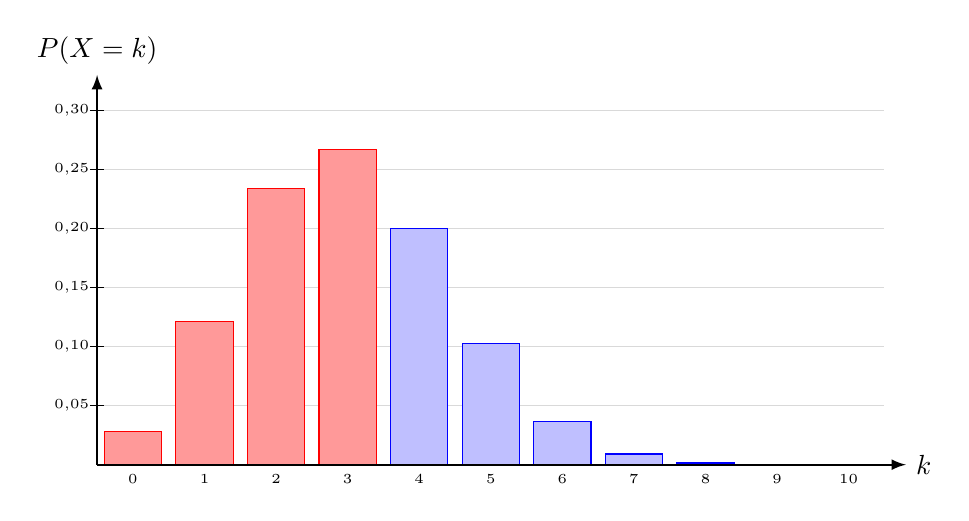
\begin{tikzpicture}[x=0.909cm, y=15.000cm]
	% waagerechte Hilfslinien
	\foreach \y in {0.05,0.10,0.15,0.20,0.25,0.30}
		\draw[gray!30, thin] (-0.5,\y) -- (10.5,\y);
	% Säulen: k/P(X=k), hervorgehoben 0 bis 3
	\foreach \k/\w in {0/0.0282, 1/0.1211, 2/0.2335, 3/0.2668, 4/0.2001, 5/0.1029, 6/0.0368, 7/0.0090, 8/0.0014, 9/0.0001, 10/0.0000} {
		\filldraw[fill=blue!25, draw=blue] (\k-0.4,0) rectangle (\k+0.4,\w);
		\ifnum\k<0 \else \ifnum\k>3 \else
			\filldraw[fill=red!40, draw=red] (\k-0.4,0) rectangle (\k+0.4,\w);
		\fi\fi
	}
	% Achsen
	\draw[-latex, thick] (-0.5,0) -- (10.8,0) node[right] {$k$};
	\draw[-latex, thick] (-0.5,0) -- (-0.5,0.330) node[above] {$P(X=k)$};
	\foreach \k in {0,...,10}
		\node[below, font=\tiny] at (\k,0) {$\k$};
	\foreach \y/\t in {0.05/0{,}05, 0.10/0{,}10, 0.15/0{,}15, 0.20/0{,}20, 0.25/0{,}25, 0.30/0{,}30}
		\draw (-0.6,\y) -- (-0.4,\y) node[left, font=\tiny, xshift=-2pt] {$\t$};
\end{tikzpicture}
\end{lstlisting}

\begin{ausgabe}
\centering
% Binomialverteilung B(10; 0{,}3) – erzeugt mit binomial_saeulen.py
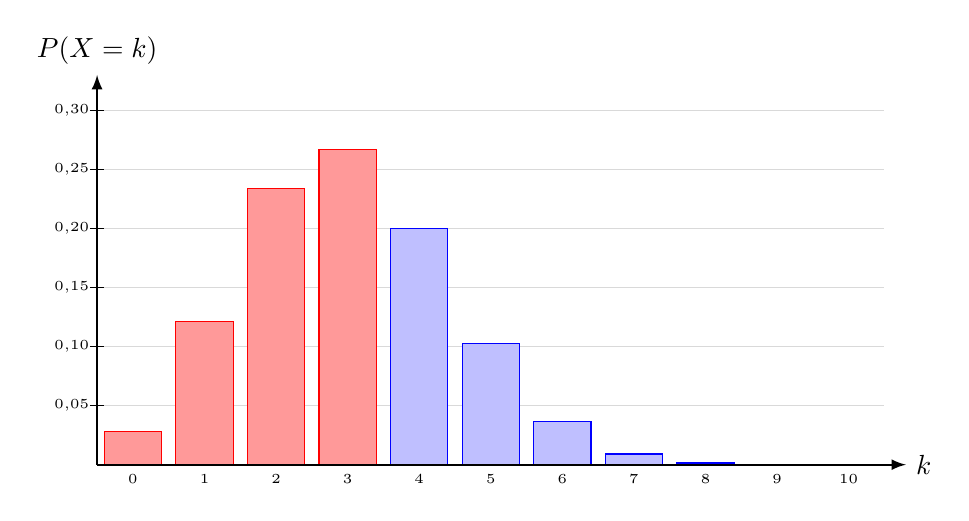
\begin{tikzpicture}[x=0.909cm, y=15.000cm]
	% waagerechte Hilfslinien
	\foreach \y in {0.05,0.10,0.15,0.20,0.25,0.30}
		\draw[gray!30, thin] (-0.5,\y) -- (10.5,\y);
	% Säulen: k/P(X=k), hervorgehoben 0 bis 3
	\foreach \k/\w in {0/0.0282, 1/0.1211, 2/0.2335, 3/0.2668, 4/0.2001, 5/0.1029, 6/0.0368, 7/0.0090, 8/0.0014, 9/0.0001, 10/0.0000} {
		\filldraw[fill=blue!25, draw=blue] (\k-0.4,0) rectangle (\k+0.4,\w);
		\ifnum\k<0 \else \ifnum\k>3 \else
			\filldraw[fill=red!40, draw=red] (\k-0.4,0) rectangle (\k+0.4,\w);
		\fi\fi
	}
	% Achsen
	\draw[-latex, thick] (-0.5,0) -- (10.8,0) node[right] {$k$};
	\draw[-latex, thick] (-0.5,0) -- (-0.5,0.330) node[above] {$P(X=k)$};
	\foreach \k in {0,...,10}
		\node[below, font=\tiny] at (\k,0) {$\k$};
	\foreach \y/\t in {0.05/0{,}05, 0.10/0{,}10, 0.15/0{,}15, 0.20/0{,}20, 0.25/0{,}25, 0.30/0{,}30}
		\draw (-0.6,\y) -- (-0.4,\y) node[left, font=\tiny, xshift=-2pt] {$\t$};
\end{tikzpicture}
\end{ausgabe}



%%%%  KAPITEL 5  %%%%
\section{Zusammenfassung}

Die wichtigsten Regeln:

\begin{itemize}
	\item Baumdiagramme mit \texttt{\textbackslash begin\{tikzpicture\}[baumdiagramm]}, Startpunkt \texttt{\textbackslash node[punkt] \{\}}
	\item erstes \texttt{child} = oberer Ast, Wahrscheinlichkeit oben mit \texttt{above}, unten mit \texttt{below}, Stil \texttt{wkeit}
	\item von oben nach unten mit \texttt{[baumdiagrammvertikal]}: erstes \texttt{child} = linker Ast, Beschriftung mit \texttt{left} bzw. \texttt{right}
	\item Dezimalkomma als \texttt{0\{,\}5}, Brüche mit \texttt{\textbackslash tfrac}
	\item Vierfeldertafel mit senkrechten Linien und \texttt{\textbackslash arraystretch} 1,6
	\item Säulendiagramme mit \texttt{binomial\_saeulen.py} erzeugen, nicht von Hand rechnen
\end{itemize}

So entstehen Stochastik-Materialien, die auf allen Blättern gleich aussehen und sich schnell an neue Aufgaben anpassen lassen.

\end{document}
